\documentclass{article}
\usepackage{graphicx} % Required for inserting image
\usepackage[utf8]{inputenc}
\usepackage{float}

\title{Mathematics -2 \\Real Life Application of Differential Equations - The Lotka Volterra Model}
\author{Vasu Kodati (B23EE1079)}
\date{29\textit{th} April 2024}

\begin{document}

\maketitle

\section{Introduction}

The Lotka-Volterra Model is a pair of first order nonlinear differential equations that seek to give a simple representation of the relationship of predator and prey in an environment. The basic concept is that, 
When there is no predator, prey can flourish. When there are predators, prey will die.\\
When there are prey, predators can live, but when there is no prey, predators will die. Here we see a tug of war between both the parties, where predator needs prey to live but consequently consumes the very thing it needs to survive. Let us assume that prey can spontaneously generate at rate $\alpha x$, and predators gradually die out at rate $\gamma y$ where 
\begin{itemize}
    \item  X represents the population of prey
    \item  Y represents the population of predators 
\end{itemize}

Hence we can model the equations like this - 

%write the equations 
\begin{equation}
    \frac{dx}{dt} = \alpha x - \beta xy 
    \end{equation}
    \begin{equation}
    \frac{dy}{dt} = \delta xy - \gamma y 
    \end{equation}
   

 



Here $\beta$ and $\delta$ are variables that represent how much each group interacts with each other. Also note that all the variables here are positive.

\section{History}
The Lotka-Volterra equations were developed independently by Alfred J. Lotka and Vito Volterra in the early 20th century. Lotka, an American mathematician, formulated the equations in 1920 to describe autocatalytic chemical reactions. Volterra, an Italian mathematician, derived similar equations in 1926 to model fish populations in the Adriatic Sea. \newline

Lotka was interested in understanding how the concentrations of reactants and products change over time in systems where the presence of one substance catalyzes the production of another. He developed a set of differential equations to describe the rates of change of these substances based on their interactions. \\

Meanwhile, Volterra was investigating the dynamics of fish populations in the Adriatic Sea. He independently derived similar equations in 1926 to model the interactions between predators (such as fish) and their prey (such as smaller fish or plankton) in ecological systems. Volterra observed cyclic fluctuations in fish populations and sought to understand the underlying mechanisms driving these oscillations. \newline

Although Lotka and Volterra approached the problem from different perspectives—Lotka from the realm of chemistry and Volterra from ecology—the equations they developed shared a common structure and mathematical form. Lotka's work laid the foundation for understanding feedback mechanisms in chemical systems, while Volterra's work provided insights into the dynamics of predator-prey relationships in ecological systems. Together, their contributions formed the basis of what is now known as the Lotka-Volterra equations, which have since become a cornerstone of mathematical ecology and population dynamics.

\section{Assumptions Made By Equation}
There are a number of assumptions that we make for this model, namely - 
\begin{itemize}


    \item The prey has ample food at all times
    \item The prey can spontaneously reproduce
    \item Rate of change of either population is proportional to its size
    \item The environment does not favor either species, both are equally likely to survive.
    \item The entire population is identical and can be described by a single variable. For example, there is no age, gender or natural cause of death. 
\end{itemize}
In pure absence of predator, the prey grows as - 
\[\frac{dx}{dt} = \alpha x\]
And in absence of prey, predator is affected as - 
\[\frac{dy}{dt} = -\gamma y\]
Their interaction causes promotion of predator and inhibition of prey but then predators die out due to lack of prey, and this cycle reverses yet again.
\section{Plots and Inferences}
\subsection{Plots of Functions}
Let us plot a population vs time graph of our equation. The values of variables are taken as follows - 

\[\alpha = 1.1\\\]
\[\beta = 0.1\]
\[\delta = 0.1\]
\[\gamma = 0.4\]
And the initial values of predator and prey are given by - 
\[x_0 = 20 (Prey)\]
\[y_0 = 7 (Predator)\]
(Values are assumed to be in the thousands)\\
The result is Figure 1.

\begin{figure}[H]
    \centering
    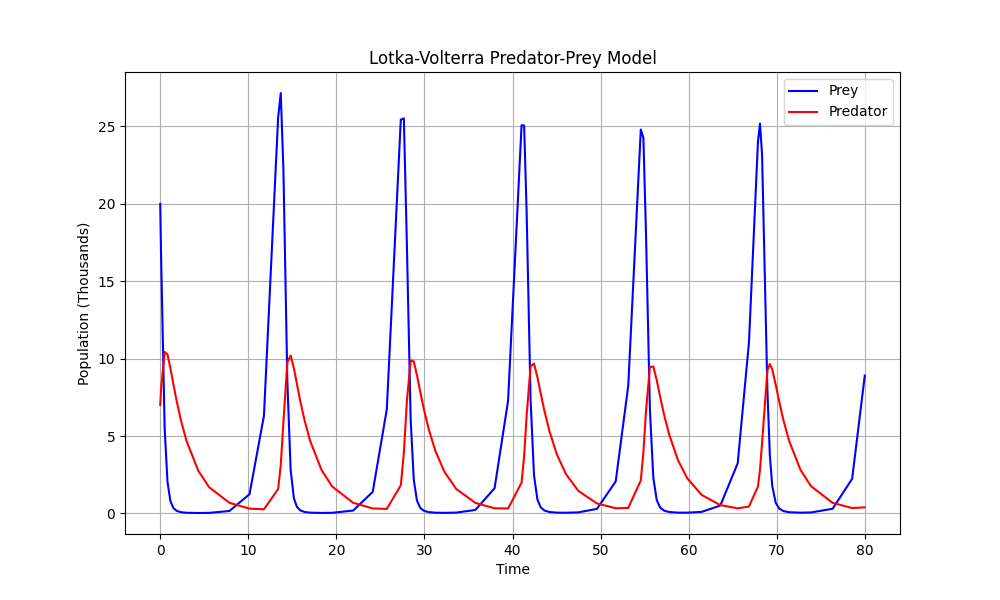
\includegraphics[width=0.75\linewidth]{LV_Time.png}
    \caption{Population vs Time Graph}
    \label{fig:1}
\end{figure}
Let us also plot a graph where the X axis is population of prey and Y axis is population of predators, where we vary the initial values of predator population. But for this, we must first eliminate the variable of time.  
\subsubsection{Creation of Phase-Space Plot}
\[\frac{dx}{dt} = \alpha x - \beta xy \]
\[\textit{dt} = \frac{dx}{\alpha x - \beta xy}\]
Similarly,
\[\frac{dy}{dt} = \delta xy - \gamma y \]
\[\textit{dt} = \frac{dy}{\delta xy - \gamma y}\]
Equating both, we get,
\[\frac{dx}{\alpha x - \beta xy} = \frac{dy}{\delta xy - \gamma y}\]
\[\frac{dy}{dx}=\frac{y}{x}\frac{(\delta x-\gamma)}{(\alpha-\beta y)}\]
\[\left(\frac{\alpha - \beta y}{y}\right)\textit{dy} =\left(\frac{\delta x - \gamma}{x}\right)\textit{dx}\]
Integrating both sides, we get 
\[\alpha \ln y - \beta y = \delta x - \gamma \ln x + C\]
\begin{equation}
    f(x,y) = \alpha \ln y + \gamma \ln x - \beta y - \delta x
\end{equation}
Now for different starting conditions, the graph of this function would look like the following:
\begin{figure}[H]
    \centering
    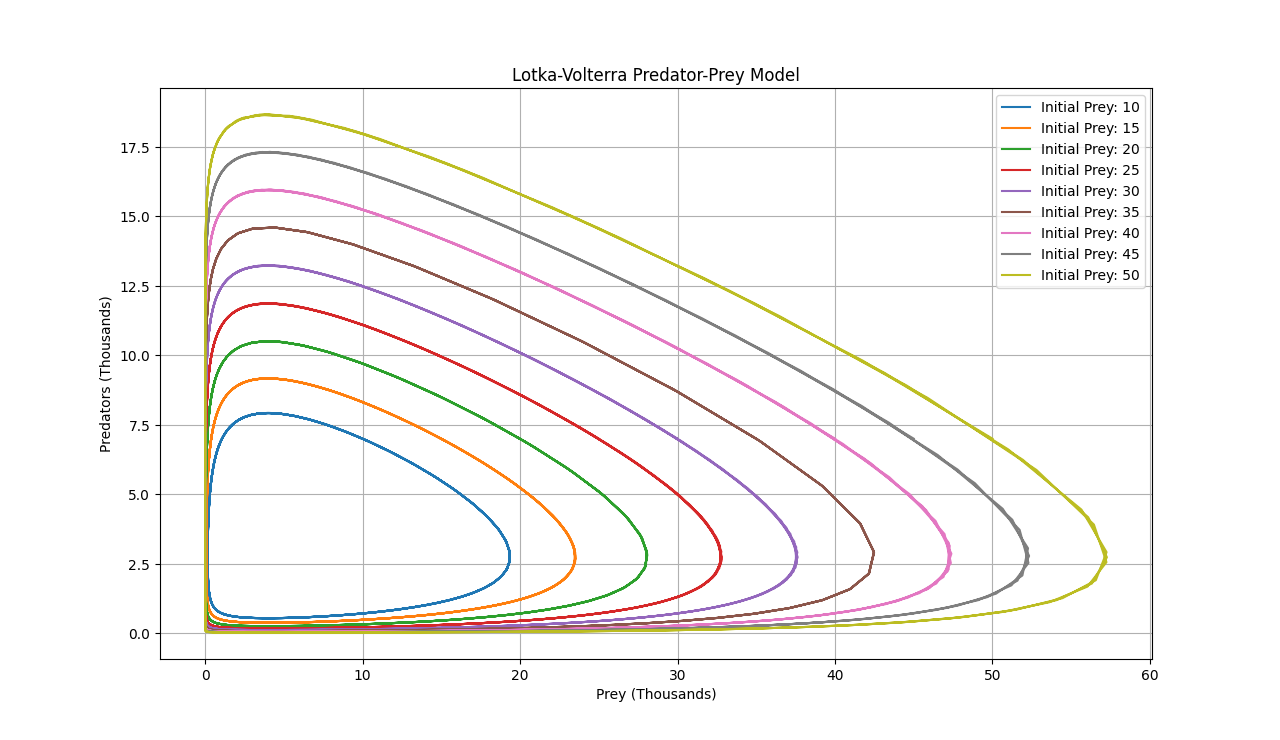
\includegraphics[width=1\linewidth]{Figure_1.png}
    \caption{Space Phase Plot of Model}
    \label{fig:2}
\end{figure}
The value of $f(x,y)$ stays constant on a given contour which represents the fluctuation of one given situation.
\subsection{Inferences from Plots}
\subsubsection{From Time Plot}
Here we can observe that as the prey population rises, so does the predator population, until the number of predators are enough such that rate of reproduction of prey is not enough to counteract the predation rate of predator. Then the population of prey goes down while predators thrive, but then predators start dying because of lack of food. And then, prey starts to reproduce enough and the cycle repeats ad infinitum.
\subsubsection{From Space Phase Plot}
From the space phase plot, we can observe that the equation yields a closed curve. Any one curve exhibits the same behaviour as the time graph if observed counter-clockwise.\newline

We can observe that the graphs are "oscillating" around a point in the bottom left of the graph. What is the significance of this point? Let us investigate this in the next section

\section{State of Equilibrium of System}
Population equilibrium occurs when both $\frac{dy}{dt}$ and $\frac{dx}{dt}$ are 0. Hence 
\[x(\alpha - \beta y) = 0\]
\[y(\delta x - \gamma) = 0\]
When solved, we get the solutions - 
\[x = y = 0\] and
\[\left(y = \frac{\alpha}{\beta}\,x = \frac{\gamma}{\delta}\right)\]
The first solutions essentially means the extinction of both species. The second represents a fixed point which both populations will always sustain their population for all of time, i.e equilibrium. Observe the following graph, where 
\[x_0 = \frac{\gamma}{\delta} = \frac{0.4}{0.1} = 4\]
\[y_0 = \frac{\alpha}{\beta} = \frac{1.1}{0.4} = 2.75\]
\begin{figure}[H]
    \centering
    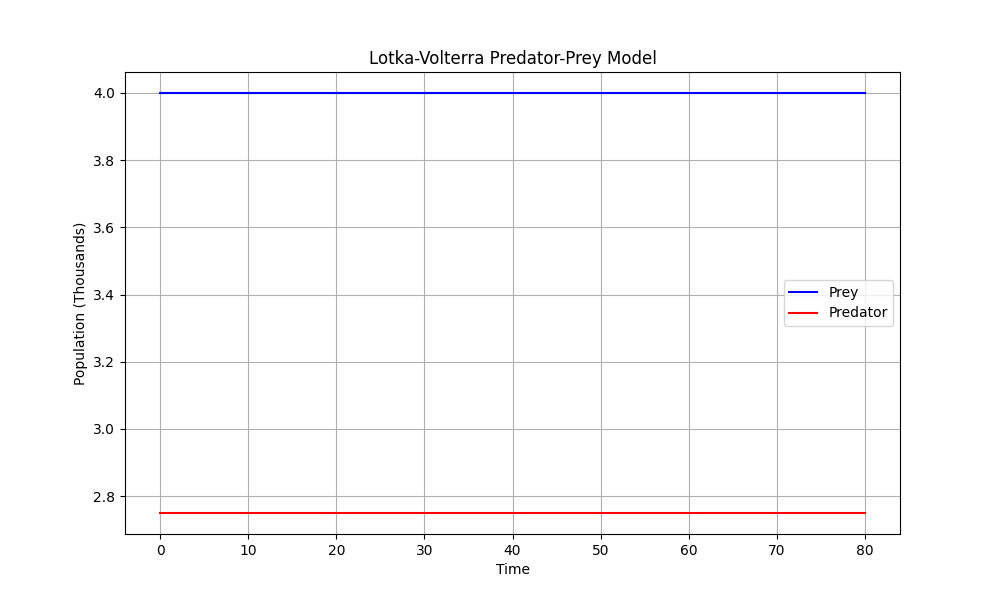
\includegraphics[width=0.75\linewidth]{LV_EQUILIB.png}
    \caption{Equilibrium Plot}
    \label{fig:equi-plot}
\end{figure}
Now the question arises, if both origin and special point are locations where derivative of system is zero, are they both stable equilibrium points? Calculating the Jacobin at both points, we see that origin is a saddle point, which is inherently unstable. This means that extinction of species in this model is quite hard. This makes sense because prey can spontaneously arise from nothingness according to this equation, hence value of prey will never be zero.
\section{Possible Improvements to System}
Along with the assumptions mentioned in Section 3,this system is  a very rudimentary implementation of biological system which omits many factors, such as- 
\begin{itemize}
    \item Resources of Environment 
    \item Diseases
    \item Random Conditions and Disasters
    \item Multiple Species and their Complex Interactions
\end{itemize}
An example of an improved model is the "Lotka Volterra Competition Model" which makes predator feeding rate proportional to prey population, making the simulation more realistic. Another improvement could be capping the population of the prey in a reasonable way since in this model, they can proliferate indefinitely.

\section{Significance of This Model}
While predominantly visualised as a predator-prey concept, this model can be expanded to many other fields, such as - 
\begin{itemize}
    \item Applied Mathematics 
    \item Interdependent Catalytic Reactions in Chemistry
    \item Disease Spread ( Pathogens as Predator, Host as Prey)
    \item Resource Management,
\end{itemize}
and so many more. \\
Overall, the Lotka-Volterra model serves as a valuable tool for understanding the dynamics of ecological systems, informing conservation efforts, and advancing our knowledge of population interactions in nature. Its simplicity and versatility make it a cornerstone of ecological and mathematical modeling.



\end{document}
